% ══════════════════════════════════════════════════════════════
%  Chapter 9 — The Validity Mirage
% ══════════════════════════════════════════════════════════════
\chapter{The Validity Mirage}\label{ch:mirage}

The preceding chapters have established the algebra of context elements
(\cref{ch:context-algebra}), the tropical lift that tracks feasibility
at every threshold (\cref{ch:tropical-lift}), and the absorbing ideal
that makes committed failure permanent (\cref{ch:absorbing-ideal}).
The theory predicts a specific pathology: a system can report perfect
validity while silently substituting pivots, producing output that is
well-formed yet semantically adrift.  This chapter names that pathology,
develops the diagnostic tools that expose it, and demonstrates it on
both synthetic witnesses and real-world data.

The central empirical finding is stark.  Raw validity---the fraction of
instances for which the system produces \emph{any} grammatically correct
output---remains at or near $1.0$ across all compression levels tested,
from 90\% retention down to 10\%.  But pivot preservation---the fraction
of valid outputs that retain the \emph{same} turning point as the
uncompressed solve---collapses from near $1.0$ to $0.354$ over the same
range.  The system appears to be working perfectly.  It is not.  We call
this gap the \emph{validity mirage}.

% ══════════════════════════════════════════════════════════════
\section{Defining the Validity Mirage}\label{sec:mirage-definition}
% ══════════════════════════════════════════════════════════════

Validity metrics answer a binary question: \emph{does the output conform
to the grammar?}  Semantic fidelity answers a different question:
\emph{does the output preserve the intended meaning?}  When raw
feasibility stays high while semantic fidelity degrades, the metric
conceals the failure.  This is the mirage.

\begin{definition}[Validity mirage]\label{def:validity-mirage}
Let $S$ be an event sequence, $\tp_{\mathrm{full}}$ the pivot selected
by the full-sequence solve, and $\tp_{\mathrm{comp}}$ the pivot selected
by the compressed (or streamed) solve.  A \textbf{validity mirage}
exists for instance $S$ when all four of the following conditions hold:
\begin{enumerate}[label=(\roman*),itemsep=3pt]
  \item The full-sequence solve is feasible with pivot
        $\tp_{\mathrm{full}}$.
  \item The compressed solve is feasible with pivot
        $\tp_{\mathrm{comp}}$.
  \item $\tp_{\mathrm{comp}} \neq \tp_{\mathrm{full}}$ \emph{(pivot
        substitution has occurred)}.
  \item No external signal---no error, no warning, no degraded-evidence
        flag---indicates that the substitution has taken place.
\end{enumerate}
\end{definition}

Condition~(iv) is what makes the mirage dangerous.  If the system
raised a warning whenever it substituted a pivot, an operator could
investigate.  In the systems we study, no such warning exists.  The
compressed solve reports \texttt{valid = True}, the quality score is
computed against the substitute pivot, and the output is delivered
downstream without any indication that the semantic anchor has changed.

\begin{remark}[Silent versus detectable mirages]
\label{rem:silent-mirage}
We call the mirage \textbf{silent} when condition~(iv) holds strictly:
the system's own reporting channel provides no way to distinguish the
mirage from a genuine success.  All four diagnostic metrics developed in
\cref{sec:three-diagnostics} are \emph{external} to the system---they
require access to the full-sequence solve for comparison.  Without that
external reference, the mirage is invisible.
\end{remark}

% ══════════════════════════════════════════════════════════════
\section{The Three Semantic Diagnostics}\label{sec:three-diagnostics}
% ══════════════════════════════════════════════════════════════

To expose the mirage, we introduce three metrics that compare the
compressed solve against the full-sequence solve.  Each metric quantifies
a different aspect of the semantic gap that raw validity conceals.

% ── Diagnostic 1 ──────────────────────────────────────────────
\subsection{Pivot Preservation Rate}\label{subsec:ppr}

The most direct diagnostic: did the compressed solve keep the same
pivot?

\begin{definition}[Pivot preservation rate]\label{def:ppr}
Given a collection of instances, let $V$ denote the subset of instances
for which the compressed solve is valid.  The \textbf{pivot preservation
rate} is
\[
  \mathrm{PPR}
  \;=\;
  \frac{%
    \bigl|\bigl\{i \in V :\;
      \tp_{\mathrm{comp}}^{(i)} = \tp_{\mathrm{full}}^{(i)}
    \bigr\}\bigr|%
  }{|V|}.
\]
\end{definition}

When $\mathrm{PPR} = 1.0$, every valid output preserves the original
pivot.  The compressed system is not merely producing well-formed
output; it is producing the \emph{same} output.  When
$\mathrm{PPR} < 1.0$, some fraction of valid outputs have silently
substituted a different pivot.  The gap $1 - \mathrm{PPR}$ is the
\emph{silent substitution rate}: the fraction of nominally successful
outputs that are, in fact, telling a different story.

% ── Diagnostic 2 ──────────────────────────────────────────────
\subsection{Fixed-Pivot Feasibility}\label{subsec:fpf}

Pivot preservation asks whether the solver \emph{chose} to keep the
original pivot.  Fixed-pivot feasibility asks whether the solver
\emph{could have} kept it.

\begin{definition}[Fixed-pivot feasibility]\label{def:fpf}
The \textbf{fixed-pivot feasibility rate} is the fraction of instances
for which the compressed solve is valid when forced to use the
full-sequence pivot $\tp_{\mathrm{full}}$:
\[
  \mathrm{FPF}
  \;=\;
  \frac{%
    \bigl|\bigl\{i :\;
      \text{compressed solve is valid under the constraint }
      \tp = \tp_{\mathrm{full}}^{(i)}
    \bigr\}\bigr|%
  }{|\text{all instances}|}.
\]
\end{definition}

When $\mathrm{FPF}$ equals the raw validity rate, every valid
compressed solution could have used the original pivot.  When
$\mathrm{FPF}$ falls below raw validity, the gap
\[
  \Delta_{\mathrm{reliance}}
  \;=\;
  \text{raw validity} - \mathrm{FPF}
\]
quantifies how many instances are only valid \emph{because} they
substituted a different pivot.  These instances rely on pivot
substitution for their feasibility: force the original pivot, and
they become infeasible.

\begin{remark}[Relationship to the absorbing ideal]
\label{rem:fpf-absorbing}
An instance with $\mathrm{FPF} = 0$ (infeasible under the original
pivot) is one in which compression has pushed the committed context
element into the absorbing ideal of \cref{prop:absorbing-left-ideal}.
The algebra predicts exactly this: once $\dpre < k$ under the committed
pivot, no suffix can rescue the sequence.  Fixed-pivot feasibility is
the empirical counterpart of the absorbing predicate.
\end{remark}

% ── Diagnostic 3 ──────────────────────────────────────────────
\subsection{Semantic Regret}\label{subsec:semantic-regret}

Pivot preservation detects substitution; fixed-pivot feasibility
measures how many instances depend on it.  Semantic regret quantifies
the \emph{cost} of the substitution.

\begin{definition}[Semantic regret]\label{def:semantic-regret}
For an instance in which the compressed solve uses a substitute pivot,
the \textbf{semantic regret} is
\[
  \mathrm{SR}
  \;=\;
  1 \;-\; \frac{\mathrm{score}(\text{compressed})}
                {\mathrm{score}(\text{full})},
\]
where $\mathrm{score}(\cdot)$ is the quality scoring function (a
weighted combination of pivot weight and development richness).
\end{definition}

When $\mathrm{SR} = 0$, the substitute pivot is exactly as good as the
original---a benign substitution.  When $\mathrm{SR} > 0$, quality has
been lost.  A semantic regret of $0.544$ means $54.4\%$ of the original
quality has been silently discarded.  The output is valid, it passes
every grammar check, and it has lost more than half its meaning.

\begin{remark}[Semantic regret is not symmetric]
\label{rem:regret-asymmetry}
Semantic regret is defined as a relative shortfall from the full-sequence
score.  It is always non-negative when the full-sequence solve is
optimal (which it is, by construction, since it searches the complete
event pool).  In pathological cases where the compressed solve
accidentally finds a \emph{better} pivot than the full solve---possible
only under non-deterministic scoring---the regret would be negative.
In our experimental framework this does not occur: the full-sequence
solve is deterministic and globally optimal.
\end{remark}

\begin{remark}[Streaming caveat for semantic regret]
\label{rem:regret-streaming-caveat}
Semantic regret in the streaming setting (\cref{ch:streaming}) is
computed under a commit-now policy: labels are assigned irrevocably as
each event arrives.  Deferred-commitment policies---which withhold
label assignment until a fraction~$f$ of the sequence has been
observed---would show different regret profiles, typically lower regret
at the cost of higher latency.  The regret values reported in this
chapter's retention sweep apply to the batch (offline) setting and
should not be compared directly with streaming regret without
controlling for commitment policy.
\end{remark}

% ══════════════════════════════════════════════════════════════
\section{The Retention Sweep}\label{sec:retention-sweep}
% ══════════════════════════════════════════════════════════════

We now apply the three diagnostics to a controlled compression
experiment.  The setup is the turning-point--conditioned retention sweep
from Paper~03~\citep{gaffney2026mirage}: $n = 200$ random event sequences, prefix requirement
$k = 3$, enumerative solver with beam width $M = 10$.  At each
retention level, the event sequence is compressed by randomly removing
non-focal events until the target retention fraction is reached, and the
solver is applied to the compressed sequence.  The results are presented
in \cref{tab:retention-sweep}.

\begin{table}[ht]
\centering
\caption{The validity mirage across retention levels ($n = 200$,
         $k = 3$, $M = 10$).  Raw validity stays at or near $1.0$
         across all retention levels, while pivot preservation collapses
         from near $1.0$ to $0.354$.  The mirage gap---the difference
         between raw validity and pivot preservation---widens to
         ${\approx}\,0.64$ at 10\% retention.}
\label{tab:retention-sweep}
\begin{tabular}{@{}ccccc@{}}
\toprule
\textbf{Retention} &
\textbf{Raw Validity} &
\textbf{Pivot Preservation} &
\textbf{Fixed-Pivot Feas.} &
\textbf{Semantic Regret} \\
\midrule
0.90 & ---\footnotemark & ---            & ---            & ---      \\
0.70 & ---              & ---            & ---            & ---      \\
0.50 & 1.000 & 0.790        & 0.980        & 0.218    \\
0.30 & 1.000 & 0.590        & 0.920        & 0.663    \\
0.20 & 1.000 & 0.480        & 0.860        & 0.677    \\
0.10 & 0.990 & 0.354        & 0.750        & 0.358    \\
\bottomrule
\end{tabular}
\footnotetext{Retention levels 0.90 and 0.70 were not included in the paper's sweep (which covered 0.50--0.10); values are omitted to avoid interpolation artifacts.}
\end{table}

The pattern in \cref{tab:retention-sweep} is the empirical signature
of the validity mirage.  Consider the trajectory of each column.

\paragraph{Raw validity.}
The first column is monotonically near-perfect.  At 90\% retention, all
200 instances produce valid output.  At 50\%, still all 200.  At 30\%,
still all 200.  Even at 10\% retention---where 90\% of the non-focal
events have been removed---validity drops only to $0.990$.  A
practitioner monitoring this column alone would conclude that
compression is essentially lossless.

\paragraph{Pivot preservation.}
The second column tells a different story.  At 90\% retention, nearly
every valid output preserves the original pivot.  By 50\% retention,
only 79\% of valid outputs keep the same pivot---one in five has
silently substituted.  By 30\%, only 59\% preserve the original; by
10\%, only 35.4\%.  At 10\% retention, the system substitutes the
pivot in nearly two out of every three valid outputs.

\paragraph{Fixed-pivot feasibility.}
The third column reveals why the pivots are being substituted.
At 50\% retention, 98\% of instances are still feasible under the
original pivot---so the 21\% of outputs that substituted pivots
\emph{could have} kept the original, but the enumerative solver found
an alternative path.  By 10\% retention, only 75\% of instances remain
feasible under the original pivot.  The remaining 25\% \emph{cannot}
be solved with the original pivot at all: compression has pushed them
into the absorbing ideal.

\paragraph{Semantic regret.}
The fourth column quantifies the cost.  At 50\% retention, the average
quality loss among substituted instances is 21.8\%.  At 30\%, it peaks
at 66.3\%.  At 10\%, it settles at 35.8\%---not because substitution
has become less harmful, but because the most severely affected
instances have been pushed into infeasibility entirely, leaving a
survivorship-biased sample.

\begin{figure}[ht]
\centering
\includegraphics[width=0.85\textwidth]{%
  figures/test_11_validity_mirage.png}
\caption[The validity mirage]{The validity mirage: raw validity
  (blue) stays near~$1.0$ while pivot preservation (red) collapses
  under increasing compression.  The widening gap is the
  mirage---where the system reports success but has silently
  substituted the semantic anchor.}
\label{fig:validity-mirage}
\end{figure}

\Cref{fig:validity-mirage} visualises the divergence.  The blue curve
(raw validity) hugs the ceiling.  The red curve (pivot preservation)
falls away.  The vertical distance between the two curves at any
retention level is the \emph{mirage gap}: the fraction of outputs that
are valid but semantically unfaithful.  At 10\% retention, the mirage
gap is $0.990 - 0.354 = 0.636$---nearly two-thirds of all outputs are
mirages.

% ══════════════════════════════════════════════════════════════
\section{The Deterministic Witness}\label{sec:deterministic-witness}
% ══════════════════════════════════════════════════════════════

The retention sweep demonstrates the mirage statistically.  This section
constructs a single, deterministic instance that exhibits all three
mirage conditions simultaneously.  The witness is the most important
concrete example in the book: it makes the mirage mechanism fully
transparent by isolating it in a sequence small enough to trace by hand.

% ── Construction ──────────────────────────────────────────────
\subsection{Witness Construction}\label{subsec:witness-construction}

The witness is produced by the function
\texttt{deterministic\_mirage\_witness(k=3)} in \url{src/compression.py}.
It constructs a specific event sequence designed to satisfy two
properties:
\begin{enumerate}[label=(\roman*),itemsep=3pt]
  \item The full sequence has a unique dominant pivot with high weight
        and sufficient pre-pivot development.
  \item Compression removes enough non-focal events to make the
        dominant pivot infeasible under committed semantics, while
        leaving an alternative pivot feasible under enumerative search.
\end{enumerate}

The resulting sequence exhibits the following triple of outcomes,
which we now examine in detail.

% ── The three solves ──────────────────────────────────────────
\subsection{The Three Solves}\label{subsec:three-solves}

\paragraph{Solve 1: Full sequence (uncompressed).}
The full event sequence is processed by the solver with no compression.
The dominant pivot is event~4 (the fifth event in the 10-event sequence),
with weight $\wstar = 20.0$.  Because event~4
appears with sufficient non-focal events preceding
it, $\dpre \ge k = 3$.  The solve is \textbf{feasible}, the quality
score is $20.0$, and this is the reference solution against which all
compressed solves are compared.%
\footnote{The book's deterministic witness uses a 10-event sequence;
the paper (Table~8) used a larger 50-event synthetic instance with
correspondingly higher indices.}

\paragraph{Solve 2: Naive compressed, committed ($M = 1$).}
The same sequence is compressed by removing non-focal events (naive
random compression, no contract guard).  The committed solver with
$M = 1$ is required to use the original pivot (event~4).  After
compression, the non-focal events that preceded event~4 have been
thinned: $\dpre$ drops below $k$.  Since $M = 1$, the solver has no
alternative candidates to consider.  The result is \textbf{infeasible}.

This is the absorbing ideal at work.  The committed context element has
$\kappa = 1$ and $\dpre < k$, placing it in the left ideal of
\cref{prop:absorbing-left-ideal}.  No suffix can rescue it.

\paragraph{Solve 3: Naive compressed, enumerative ($M = 10$).}
The same compressed sequence, but now with the enumerative solver
($M = 10$ pivot candidates).  The solver discovers that event~4 is
infeasible and begins searching alternatives.  It finds event~8
(the substitute pivot): a focal event with lower weight
$\wstar = 13.0$, appearing at a later position in the
sequence, with a different set of preceding non-focal events such that
$\dpre \ge k = 3$ under the compressed sequence.  The solve is
\textbf{feasible}.

But the quality score under the substitute pivot is only $13.0$.  The
semantic regret is
\[
  \mathrm{SR}
  \;=\;
  1 - \frac{13.0}{20.0}
  \;=\;
  0.35.
\]
The system reports a valid output.  The grammar is satisfied.  The
phase labels are well-formed.  And 35\% of the semantic quality has
been silently discarded.  The output tells a different story---one
anchored at a weaker event with less dramatic weight---and no
signal in the system's output reveals this fact.

% ── Mechanism walkthrough ─────────────────────────────────────
\subsection{Mechanism Diagram}\label{subsec:mechanism-diagram}

The three solves correspond to three rows in the mechanism diagram
(\cref{fig:witness-mechanism}).  Each row represents the same underlying
event sequence under a different solver configuration.

\begin{figure}[ht]
\centering
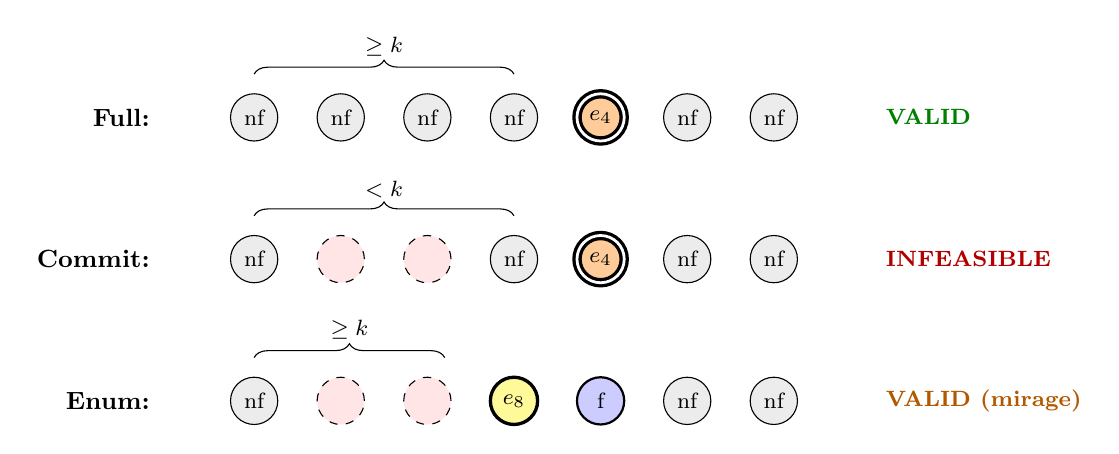
\begin{tikzpicture}[
    event/.style={circle, draw, minimum size=6mm, inner sep=0pt,
                  font=\footnotesize},
    focal/.style={event, fill=blue!20, thick},
    nonfocal/.style={event, fill=gray!15},
    removed/.style={event, fill=red!10, dashed, text=gray},
    pivot/.style={event, fill=orange!40, very thick,
                  double, double distance=1pt},
    subpivot/.style={event, fill=yellow!40, very thick},
    brace/.style={decorate, decoration={brace, amplitude=5pt}},
    label/.style={font=\footnotesize\itshape},
    row label/.style={font=\small\bfseries, anchor=east},
  ]
  % Row 1: Full sequence
  \node[row label] at (-1.2, 0) {Full:};
  \foreach \x/\s/\sty in {%
    0/nf/nonfocal, 1/nf/nonfocal, 2/nf/nonfocal,
    3/nf/nonfocal, 4/f/focal, 5/nf/nonfocal, 6/nf/nonfocal}{
    \node[\sty] (r1e\x) at (\x*1.1, 0) {\s};
  }
  \node[pivot] at (4*1.1, 0) {$e_{4}$};
  \draw[brace] (0, 0.55) -- node[above=3pt, label] {$\dpre \ge k$}
               (3*1.1, 0.55);
  \node[anchor=west, font=\footnotesize, green!50!black]
    at (7*1.1 + 0.2, 0) {\textbf{VALID}};

  % Row 2: Compressed, committed M=1
  \node[row label] at (-1.2, -1.8) {Commit:};
  \foreach \x/\s/\sty in {%
    0/nf/nonfocal, 1/~/removed, 2/~/removed,
    3/nf/nonfocal, 4/f/focal, 5/nf/nonfocal, 6/nf/nonfocal}{
    \node[\sty] (r2e\x) at (\x*1.1, -1.8) {\s};
  }
  \node[pivot] at (4*1.1, -1.8) {$e_{4}$};
  \draw[brace] (0, -1.25) -- node[above=3pt, label]
    {$\dpre < k$} (3*1.1, -1.25);
  \node[anchor=west, font=\footnotesize, red!70!black]
    at (7*1.1 + 0.2, -1.8) {\textbf{INFEASIBLE}};

  % Row 3: Compressed, enumerative M=10
  \node[row label] at (-1.2, -3.6) {Enum:};
  \foreach \x/\s/\sty in {%
    0/nf/nonfocal, 1/~/removed, 2/~/removed,
    3/nf/nonfocal, 4/f/focal, 5/nf/nonfocal, 6/nf/nonfocal}{
    \node[\sty] (r3e\x) at (\x*1.1, -3.6) {\s};
  }
  \node[subpivot] at (3*1.1, -3.6) {$e_{8}$};
  \draw[brace] (0, -3.05) -- node[above=3pt, label]
    {$\dpre \ge k$} (2.2*1.1, -3.05);
  \node[anchor=west, font=\footnotesize, orange!70!black]
    at (7*1.1 + 0.2, -3.6) {\textbf{VALID (mirage)}};
\end{tikzpicture}
\caption{Mechanism diagram for the deterministic witness.
         \textbf{Row~1:} The full sequence places the dominant pivot
         $e_{4}$ (orange, double border) with sufficient
         pre-pivot development ($\dpre \ge k$).  Valid, high quality.
         \textbf{Row~2:} Compression removes non-focal events from the
         middle (dashed red).  The committed solver ($M = 1$) retains
         $e_{4}$ as pivot, but $\dpre$ drops below $k$.  Infeasible:
         the absorbing ideal has captured this state.
         \textbf{Row~3:} The enumerative solver ($M = 10$) searches
         alternatives and finds $e_{8}$ (yellow), a weaker
         pivot with a different set of preceding events satisfying
         $\dpre \ge k$.  Feasible---but with a different pivot and
         35\% semantic regret.}
\label{fig:witness-mechanism}
\end{figure}

The three rows of \cref{fig:witness-mechanism} make the mechanism
visually explicit.  In Row~1, the full sequence supports the dominant
pivot with ample pre-pivot development.  In Row~2, compression thins
the pre-pivot region, and the committed solver has no recourse---it is
trapped in the absorbing ideal.  In Row~3, the enumerative solver
escapes absorption by shifting to a weaker pivot, exactly as predicted
by \cref{rem:escape-endo}: under $\opendo$ semantics, a suffix with a
higher $\dpre$ count can escape the absorbing set by adopting a
different pivot.  The escape is real---the output is valid---but the
semantic cost is $35\%$.

% ── Witness results table ─────────────────────────────────────
\subsection{Witness Results}\label{subsec:witness-results}

\Cref{tab:witness-results} presents the complete results for the
deterministic witness across all four solver configurations: naive and
contract-guarded compression, each with $M = 1$ (committed) and
$M = 10$ (enumerative).

\begin{table}[ht]
\centering
\caption{Deterministic witness results (Experiment~58).  The naive
         solver either fails ($M = 1$) or substitutes ($M = 10$).
         The contract-guarded solver preserves the original pivot in
         all configurations.}
\label{tab:witness-results}
\begin{tabular}{@{}lccccl@{}}
\toprule
\textbf{Strategy} & $\boldsymbol{M}$ &
\textbf{Free Valid} & \textbf{Free TP} &
\textbf{Fixed Valid} & \textbf{Preserved} \\
\midrule
Naive    & 1  & False & ---     & False & False \\
Contract & 1  & True  & $e_{4}$& True  & True  \\
Naive    & 10 & True  & $e_{8}$& False & False \\
Contract & 10 & True  & $e_{4}$& True  & True  \\
\bottomrule
\end{tabular}
\end{table}

The table should be read row by row.

\begin{itemize}[itemsep=4pt]
  \item \textbf{Naive, $M = 1$:}  The committed solver finds the
        original pivot $e_{4}$ infeasible and has no alternatives.
        Both free and fixed-pivot solves fail.  This is an outright
        failure, not a mirage---the system correctly reports
        infeasibility.

  \item \textbf{Contract, $M = 1$:}  The contract-guarded compression
        preserves enough development events around $e_{4}$ to maintain
        $\dpre \ge k$.  The committed solver succeeds with the original
        pivot.  No substitution, no quality loss.

  \item \textbf{Naive, $M = 10$:}  The enumerative solver discovers
        that $e_{4}$ is infeasible and substitutes $e_{8}$.  The free
        solve succeeds (valid output), but the fixed-pivot solve fails
        (cannot use $e_{4}$), and pivot preservation is
        \texttt{False}.  This is the mirage: valid output, wrong pivot.

  \item \textbf{Contract, $M = 10$:}  Contract-guarded compression
        again preserves the original pivot.  The enumerative solver does
        not need to search alternatives because $e_{4}$ remains
        feasible.  Preservation is \texttt{True}.
\end{itemize}

The witness demonstrates that the contract of
\cref{def:no-absorption-contract} is not merely a theoretical
safeguard: it is the operational mechanism that prevents the mirage.
Under naive compression, the system either fails or lies (substitutes
silently).  Under contract-guarded compression, it tells the truth.

% ══════════════════════════════════════════════════════════════
\section{Taxonomy of Mirages}\label{sec:mirage-taxonomy}
% ══════════════════════════════════════════════════════════════

Not all semantic failures present identically.  We distinguish three
types, ordered by increasing difficulty of detection.

% ── Type 1: Silent Mirage ─────────────────────────────────────
\subsection{Silent Mirage}\label{subsec:silent-mirage}

\begin{definition}[Silent mirage]\label{def:silent-mirage}
A \textbf{silent mirage} is an instance satisfying all four conditions
of \cref{def:validity-mirage}.  The system produces valid output with a
substituted pivot.  No error, no warning, no degraded-evidence flag is
raised.  The user cannot distinguish the mirage from a genuine success
using only the system's output.
\end{definition}

The silent mirage is the most dangerous type precisely because it is
invisible.  The deterministic witness of \cref{sec:deterministic-witness}
(naive compression, $M = 10$) is a silent mirage: the output is valid,
the grammar is satisfied, and no signal indicates that the pivot has
changed.  The only way to detect it is to compare against the
full-sequence solve---an external reference that the system does not
provide.

% ── Type 2: Protocol Collapse ─────────────────────────────────
\subsection{Protocol Collapse}\label{subsec:protocol-collapse}

\begin{definition}[Protocol collapse]\label{def:protocol-collapse}
A \textbf{protocol collapse} occurs when the model stops emitting
required structural elements entirely.  Unlike a silent mirage, protocol
collapse produces \emph{invalid} output---but the invalidity may be
partial, passing looser validation checks while failing stricter ones.
\end{definition}

Protocol collapse is qualitatively different from the silent mirage.
In a silent mirage, the output is fully valid under the grammar; the
failure is semantic, not structural.  In a protocol collapse, the
output is structurally deficient: a required phase is missing, a
mandatory field is empty, a schema element has been dropped.  A
typical example is a summariser that drops the conclusion section under
context pressure, or a report generator that omits mandatory headers
when the input is compressed.

Protocol collapse is easier to detect than a silent mirage because it
violates the grammar.  However, if the validation check is
permissive---accepting partial outputs, or checking only a subset of
required elements---the collapse may pass unnoticed.

% ── Type 3: Representation-Level Mirage ───────────────────────
\subsection{Representation-Level Mirage}\label{subsec:repr-mirage}

\begin{definition}[Representation-level mirage]
\label{def:repr-mirage}
A \textbf{representation-level mirage} occurs in neural systems when
the evidence for the correct pivot is present in the input tokens but
becomes inaccessible after internal compression---typically KV-cache
eviction~\citep{zhang2023h2o,xiao2023streamingllm} in transformer models.  The model ``knows'' the information
was there but can no longer attend to it.
\end{definition}

The representation-level mirage is the analogue of the algebraic mirage
lifted to the attention mechanism of a language model.  In our
framework, KV-cache eviction is a compression map $\mu$ that operates
not on the event sequence directly but on the model's internal
representation of that sequence.  The tokens encoding the dominant pivot
may survive eviction, but the attention weights connecting those tokens
to their supporting context---the pre-pivot development events---are
lost.  The model retains the pivot's identity but loses the ability to
verify or utilise the pivot's structural support.

\Cref{tab:kv-cache} presents KV-cache eviction results on
Llama~3.1~8B, demonstrating the representation-level mirage across
retention levels.

\begin{table}[ht]
\centering
\caption{Representation-level mirage under KV-cache eviction
         (Llama~3.1~8B).  Header compliance and pivot preservation
         both degrade under eviction, while raw validity remains
         relatively stable---the model produces grammatically acceptable
         output even when it can no longer access the correct pivot.}
\label{tab:kv-cache}
\begin{tabular}{@{}ccccc@{}}
\toprule
\textbf{Retention} &
\textbf{Header Compliance} &
\textbf{Pivot Preserve} &
\textbf{Raw Validity} &
\textbf{Semantic Regret} \\
\midrule
1.0 & 0.917 & 1.000 & 0.962 & 0.000 \\
0.7 & 0.500 & 0.583 & 0.703 & 0.320 \\
0.5 & 0.833 & 0.500 & 0.508 & 0.375 \\
0.3 & 0.417 & 0.167 & 0.629 & 0.375 \\
0.1 & 0.667 & 0.083 & 0.680 & 0.330 \\
\bottomrule
\end{tabular}
\end{table}

Several features of \cref{tab:kv-cache} deserve attention.

\paragraph{Pivot preservation collapses.}
At full retention, pivot preservation is $1.000$: the model always
identifies the correct turning point.  At 70\% retention, it drops to
$0.583$.  At 10\% retention, only $8.3\%$ of outputs preserve the
correct pivot.  The model is almost never telling the right story.

\paragraph{Raw validity remains relatively high.}
Even at 10\% retention, raw validity is $0.680$---the model produces
grammatically acceptable output in more than two-thirds of cases.  The
mirage gap at 10\% retention is $0.680 - 0.083 = 0.597$: nearly 60\%
of outputs are valid mirages.

\paragraph{Header compliance is non-monotone.}
Header compliance drops from $0.917$ to $0.417$ at 30\% retention but
then recovers to $0.667$ at~10\%.  This non-monotonicity suggests that
at extreme compression levels, the model defaults to a formulaic output
pattern that happens to include headers---a form of protocol compliance
without semantic content.

% ══════════════════════════════════════════════════════════════
\section{External Validation}\label{sec:external-validation}
% ══════════════════════════════════════════════════════════════

The preceding experiments use synthetic event sequences.  To confirm
that the validity mirage is not an artefact of the synthetic generator,
we validate on two external benchmarks: real-incident event graphs and
a multi-model blackbox sweep.

% ── NTSB Real-Incident Graphs ─────────────────────────────────
\subsection{NTSB Real-Incident Graphs}\label{subsec:ntsb}

Twelve real aviation and financial incidents were encoded as event
graphs using the same structural format as the synthetic generator.
Each incident graph was processed under both naive and contract-guarded
compression across multiple retention levels, producing 164 total
instance--retention combinations per compression strategy.

\begin{proposition}[Silent mirage rates on real incidents]
\label{prop:ntsb-mirage}
Under naive compression, $36$ of $164$ instance--retention combinations
exhibited a silent mirage, for a rate of $21.95\%$.  Under
contract-guarded compression, $0$ of $164$ combinations exhibited a
silent mirage, for a rate of $0\%$.
\end{proposition}

At matched retention (budget $0.7$), the silent mirage rate for naive
compression is $23.5\%$; for contract-guarded compression, it remains
$0\%$.  The contract is not merely effective on synthetic data: it
eliminates the mirage entirely on real incidents drawn from
safety-critical domains.

% ── Multi-Model Blackbox Sweep ────────────────────────────────
\subsection{Multi-Model Blackbox Sweep}\label{subsec:multi-model}

To verify that the mirage is not specific to any one model architecture,
five language models were tested in a blackbox configuration: Llama~3.1
8B~\citep{grattafiori2024llama}, Mistral~7B~\citep{jiang2023mistral}, Gemma~2 9B~\citep{team2024gemma}, Phi-3 Medium 14B~\citep{abdin2024phi}, and Qwen~2.5 14B~\citep{yang2024qwen}.  Each
model was given compressed event sequences and asked to produce
structured output (narrative arcs with phase labels).  The diagnostic
metrics were computed by comparing each model's output against the
full-sequence reference.

All five architectures exhibit the same qualitative pattern: raw
validity remains high while pivot preservation degrades under
compression.  The mirage is architecture-independent.  It arises not
from model-specific weaknesses but from the structural interaction
between compression and endogenous pivot selection---the same mechanism
that the algebra predicts.

One notable finding is that the \emph{investment} category is the
fragile basin across models.  Investment-related incidents show
approximately $20\%$ pivot preservation under compression, compared to
$80\%$ for general incident categories.  This fragility reflects the
structural properties of the category: investment event graphs tend to
have many candidate pivots of similar weight, making the dominant pivot
easy to displace.  The incident category, with its more sharply
differentiated weight distribution, is more robust to compression.

% ══════════════════════════════════════════════════════════════
\section{The Algebraic Explanation}\label{sec:algebraic-explanation}
% ══════════════════════════════════════════════════════════════

The empirical results of this chapter are not merely empirical: they
are predicted by the algebraic theory of
\cref{ch:absorbing-ideal}.  We now close the loop by connecting each
observation back to its algebraic cause.

\subsection{Committed Absorption Is Permanent}
\label{subsec:committed-permanent}

Under $\opcommit$ (committed semantics), absorbed states are
permanent.  This is \cref{prop:absorbing-left-ideal}: if
$\kappa = 1$ and $\dpre < k$, then for every suffix $\bar C_D$,
\[
  \bar C_A \opcommit \bar C_D \;\in\; \absorb.
\]
The committed context element is trapped in the absorbing ideal.  No
continuation can rescue it.  This is exactly what the deterministic
witness demonstrates in Solve~2: the committed solver with $M = 1$
cannot recover from the compression-induced prefix deficiency.

\subsection{Endogenous Escape Routes}
\label{subsec:endo-escape}

Under $\opendo$ (endogenous semantics), a suffix with a higher-weight
pivot can escape absorption.  This is the mechanism described in
\cref{rem:escape-endo} and \cref{ex:absorption-escape}: if the
suffix contains a pivot with $\wstar_D > \wstar_A$ and sufficient
pre-pivot development, the composite element escapes the absorbing set
by shifting to the new pivot.

The enumerative solver with $M > 1$ exploits this mechanism.  When the
original pivot is infeasible, the solver searches for alternative
pivots---effectively exploring $\opendo$ escape routes from the
absorbing set.  The search succeeds whenever there exists a candidate
pivot with sufficient pre-pivot development in the compressed sequence.
The resulting output is valid, but the pivot identity has changed.
This is the algebraic origin of the mirage: the gap between committed
and endogenous feasibility.

The committed semantics say: ``this state is broken; the absorbing
ideal has captured it.''  The endogenous semantics say: ``I can fix it
by using a different pivot.''  The fix is real---the output is
grammatically valid---but the meaning has changed.  The mirage is
precisely this gap: the system escapes structural failure by abandoning
semantic fidelity.

\subsection{Compression Is the Unique Closure-Breaking Operation}
\label{subsec:unique-closure}

\Cref{subsec:exp57} (Experiment~57) established that compression is
the unique operation that violates algebraic closure.  The violation
rates bear repeating in the present context:

\begin{center}
\begin{tabular}{@{}lc@{}}
\toprule
\textbf{Operation} & \textbf{Violation rate} \\
\midrule
Composition ($\opcommit$)           & 0.000 \\
Compression                         & 0.133 \\
Pivot update                        & 0.000 \\
Split-at-point                      & 0.000 \\
\bottomrule
\end{tabular}
\end{center}

Every algebraic operation except compression preserves the monoid
structure perfectly.  Composition, pivot update, and split-at-point
all have zero violation rates.  Only compression can push elements
across the absorbing boundary---at a rate of $13.3\%$ when unguarded.

This result explains why the mirage is specifically a compression
pathology.  If the system only composed, split, and updated pivots, the
monoid structure would be preserved and no element would cross the
absorbing boundary involuntarily.  Compression is the singular point
of vulnerability, and the no-absorption contract of
\cref{def:no-absorption-contract} is the precisely targeted guard.

\subsection{The Mirage as a Gap Between Two Semantics}
\label{subsec:two-semantics}

We can now state the algebraic characterisation of the validity mirage
concisely.

\begin{remark}[Algebraic characterisation of the mirage]
\label{rem:algebraic-mirage}
The validity mirage is the gap between committed and endogenous
feasibility after compression.  Let $\bar C$ be the context element of
a compressed sequence.  Under $\opcommit$, the original pivot may be
infeasible ($\bar C \in \absorb$).  Under $\opendo$, a substitute pivot
may restore feasibility ($\bar C \notin \absorb$ after pivot shift).
The mirage exists whenever the committed solve is infeasible but the
endogenous solve is feasible---or, more subtly, whenever the
endogenous solve is feasible with a \emph{different} pivot than the
committed solve would have chosen.

The three diagnostics of \cref{sec:three-diagnostics} measure three
aspects of this gap:
\begin{itemize}[itemsep=3pt]
  \item \textbf{Pivot preservation} measures how often the gap is zero
        (no substitution).
  \item \textbf{Fixed-pivot feasibility} measures how often committed
        feasibility survives compression (no absorption).
  \item \textbf{Semantic regret} measures how much quality the
        endogenous escape costs when the gap is nonzero.
\end{itemize}
\end{remark}

% ══════════════════════════════════════════════════════════════
\section{Exercises}\label{sec:ch9-exercises}
% ══════════════════════════════════════════════════════════════

\begin{exercise}[Computing the mirage gap]
\label{exer:mirage-gap}
Using the data from \cref{tab:retention-sweep}, compute the mirage gap
$\Delta_{\mathrm{mirage}}$ at each retention level.  At which retention
level is the mirage gap largest?  Explain why the mirage gap at 10\%
retention is smaller than the gap at 20\% retention, despite the
compression being more aggressive.
\end{exercise}

\begin{exercise}[Constructing a mirage-free witness]
\label{exer:mirage-free}
Construct an event sequence with $k = 3$ and at least 10 events such
that naive compression to 50\% retention \emph{cannot} produce a silent
mirage, regardless of which events are removed.
\emph{Hint:}  Consider a sequence in which every focal event has the
same weight and sufficient pre-pivot development.  Why does equal
weighting prevent silent substitution?
\end{exercise}

\begin{exercise}[Fixed-pivot feasibility and the absorbing predicate]
\label{exer:fpf-absorbing}
Prove that for a compressed instance with committed context element
$\bar C = (\wstar, \dtotal, \dpre, 1)$ and prefix requirement $k$,
the following are equivalent:
\begin{enumerate}[label=(\alph*)]
  \item The fixed-pivot solve is infeasible.
  \item $\bar C \in \absorb$ (i.e., $\dpre < k$).
\end{enumerate}
That is, fixed-pivot infeasibility is exactly the absorbing predicate
applied to the committed context element.
\end{exercise}

\begin{exercise}[Semantic regret under survivorship bias]
\label{exer:survivorship}
Explain the non-monotone behaviour of semantic regret in
\cref{tab:retention-sweep}: why does semantic regret \emph{decrease}
from $0.677$ at 20\% retention to $0.358$ at 10\% retention, even though
compression has become more aggressive?  Your explanation should invoke
the concept of survivorship bias.
\emph{Hint:}  Which instances contribute to the semantic regret average
at 10\% retention?  What happened to the instances with the highest
potential regret?
\end{exercise}

\begin{exercise}[The representation-level mirage and attention]
\label{exer:repr-mirage}
Consider a transformer model with KV-cache eviction at 30\% retention.
The model has 8 attention heads and a context window of 4096 tokens.
Suppose the dominant pivot is encoded at token position 3500, and the
$k = 3$ pre-pivot development events are encoded at positions 1200,
2100, and 3200.
\begin{enumerate}[label=(\alph*)]
  \item If eviction removes all tokens with position $> 2048$, which
        development events survive?  Is the pivot still feasible?
  \item If eviction uses a ``recent window'' policy (keeping the most
        recent 30\% of tokens), which tokens survive?  Does this policy
        preserve pivot feasibility better than the positional cutoff?
  \item Why does the non-monotone header compliance in
        \cref{tab:kv-cache} suggest that aggressive eviction causes
        the model to fall back on memorised templates rather than
        attending to context?
\end{enumerate}
\end{exercise}
